\section{Implementation and Performance}
\label{sec:implementation}
% We present ARLayout, a mobile tool that provides a re-layout experience in usage scenarios with AR.
% We begin by describing a generic workflow in usage scenarios. Then, we summarize the implementation points involved based on this workflow, combined with the experimental usage scenarios, and we introduce the design details of each section below.

An implementation overview of the implementation workflow
and the details are described in this section.


\begin{figure}[htp]
%\setlength{\abovecaptionskip}{0.05cm}
%\setlength{\belowcaptionskip}{-0.4cm}
    % \centering
    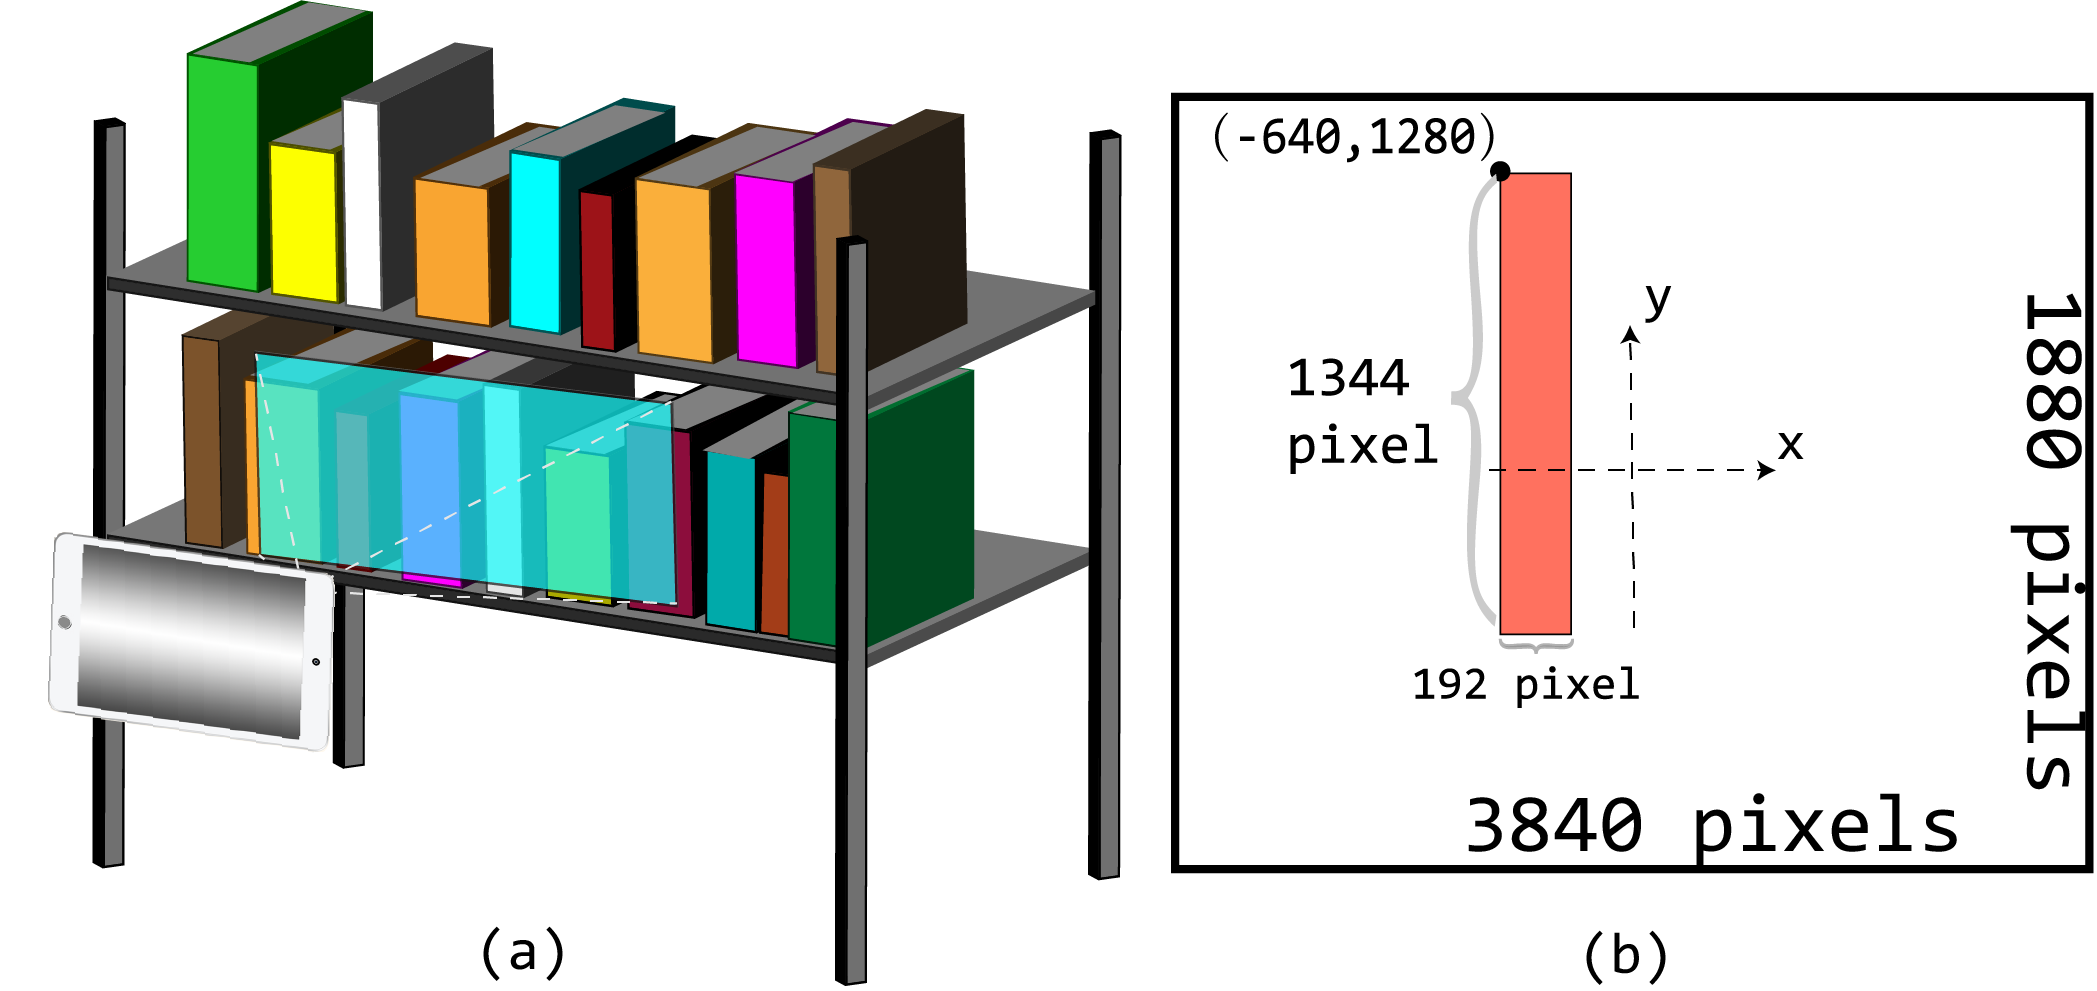
\includegraphics[width=\linewidth]{images/implementation_front.eps}
    \caption{
        (a) shows a mobile device is scanning the bookshelves.
        (b) is the top view of (a) showing the horizontal view angle $\alpha$,
        where $d$ is the distance between the mobile device and the target books estimated by \textit{ARLayout},
        and $x$ is the number of pixels horizontally.
        (c) shows a segmented book sample with the extracted position and size. %3840*1880
        % The coordinates of the top left corner of the book is (-640, 1280).
        (d) there are five blocks with recognized coffee names on a coffee menu.
    }
    \label{fig:implementation_front}
\end{figure}




%\subsection{Implementation}
%
%\textit{ARLayout} is based on C/S architecture
%that allows users to take photos/record videos in a cluttered environment
%using a mobile device such as iPad or other tablets.
%% The remote server processes the images in real-time, calculates the corresponding data feedback, and displays them by ARLayout.
%We tried \textit{ARLayout} in library, coffee shop, and cosmetics shop,
%three usage scenarios, where the objects will be
%re-grouped and re-ranked in AR space, and generate various augmented visual presentations.


\subsection{Database}

We create a large database on the server for
three application scenarios to serve these scenarios that
require real-time information feedback~\cite{Mcauley2015, He2016}.
% Some of this data is in the scenario itself, such as the title of the book, the name of the coffee, the price, and some of it is not in the scenario, but is related to the objects in the scenario, such as the book’s evaluation, the composition of the coffee.
Considering the additional information, the tool can better achieve design goal G4,
providing visual presentations or personalized recommendations by accessing the database in realtime.

% \textbf{Global Book Database}
% A database of more than 2 million books is created on the server, making it easy to quickly find the ISBN, title, author, author introduction, abstract, publisher, cover image, pages, prices, tags, ratings, reviews, etc.
% The dataset comes from jmcauley.ucsd.edu/data/Amazon/.

% The dataset comes from jmcauley.ucsd.edu/data/Amazon/, containing product reviews and metadata from Amazon, including 143.7 million reviews spanning May 1996 - July 2014. It includes reviews (ratings, text, helpfulness votes), product metadata (descriptions, category information, price, brand, and image features), and links (also viewed/also bought graphs).

% This means that we are only building a global database of books, but our application scenario is not limited to this. In similar application scenario, \textit{ARLayout} can also provide other data support through pattern matching algorithm. In other words, an interface for fast data import can be implemented in future work to meet the data service requirements of more scenarios. We will continue this topic in the Discussion section.

% \textbf{Coffee/Cosmetics Database}
% These two databases are created by the Web crawler, which crawled collection from well-known coffee, cosmetics brand website.
% For example, coffee data comes from Starbucks, including the coffee’s name, description, ingredients list, preview image, process introduction, while eyeshadow data mainly comes from Dior, including eyeshadow color, eye shape, location, use steps, tips, recommendations.

\subsection{Optical Character Recognition}


In the actual applications,
we found that the traditional OCR methods are not available for some complex scenarios,
e.g. slanted texts (\autoref{fig:implementation_ocr} (a)), %artistic fonts (\autoref{fig:implementation_ocr} (e)),
different text alignments in different languages (\autoref{fig:implementation_ocr} (c) and (d)).
The problems are that the English book texts (\autoref{fig:implementation_ocr} (c)) are often aligned in a vertical direction,
while the Chinese book texts (\autoref{fig:implementation_ocr} (d)) are often aligned in a horizontal direction.

In our experiments,
we improve the traditional OCR method, following a language adaptive design~\cite{Ling2018},
to achieve a large amount of the text characters over massive targets in reality.
In the approach, the texts of a book can be calibrated first if they are slanted,
and the language of a book will be identified first then the corresponding OCR
directions will be estimated,
which make the OCR recognition much more robust and scalable in the applications in reality.

%\textbf{Augmented OCR Network for Specific Scenarios}.
%Augmented template recognition works well when the texts are aligned well,
%e.g. the menu in a coffee shop.
%In the process of text recognition,
%the recognition template and classifier can be created according to different scenarios adaptively,
%which can automatically classify any regular format
%and output the recognition result in a structured way.
%In this section, there are two regions need to be settled.
%
%Reference region: the region pixels with fixed positions and contents
%in different pictures was chosen as anchor points of the picture,
%which can be used for template matching and rectification,
%as shown in~\autoref{fig:implementation_ocr} (f).
%Identification region: as shown in~\autoref{fig:implementation_ocr} (g),
%a field in a picture that needs to be identified
%was named to form a ``Key: Value'' relationship for ``Field name:
%Identification area content'',
%used to structurally identify the text contents.
%%of the same position of the same layout picture in real scenario.


\subsection{Image Segmentation and Labelling}

AR can effectively help users to migrate augmented information scenario
to real-world scenarios for observation.
Therefore, we use the method of image segmentation,
to help us segment and label the components from the image,
and then visualize the individual components in AR devices.
% In the actual implementation process, we sequential used the following methods to implement this function.

% \begin{figure}[htp]
%     \centering
%     \includegraphics[width=\linewidth]{images/BFS.eps}
%     \caption{
%         % (a) and (b) illustrate the process of BFS. In this image, each time the BFS cuts out the spine of a book.
%         (a) is the original photograph.
%         (b) is a single BFS expansion based on the pixel RGB values.
%         % (c) , (d) and (e) present scenarios that will have an negative impact on the effect.
%         (c) has several books of similar color, if they are adjacent, and the gap is very small, it may be considered as the same book.
%         (d) has a line between light and shadow in a shot, which can cause a book to be cut in half in poor lighting conditions.
%         (e) has a book with a color gap in its spine, and in real scenario it is possible that only the white parts are cut out.
%     }
%     \label{fig:BFS}
% \end{figure}

% \textbf{Breadth First Search}
% The algorithm was originally used for spine recognition in library/bookstore scenario. It is based on a basic assumption: the pixels at the spine of the book are basically continuous in RGB value. Therefore, on the basis of OCR, we approximate extend each text area with BFS algorithm until the pixel color transition too large, as shown in~\autoref{fig:BFS} (a) and (b). To show this process more clearly here, we have high-pixelated an area of the image. In real scenario, pixels extend by a much smaller step size (about 20 pixels per step, or 1/10 the size of the image). In the image, the green bolded edge points represent the current starting point, and the green unbolded edge points represent the feasible points that asingle BFS extension will reach. And the red points, represents the expanded RGB changes too large point. After a single BFS, all green points with unbolded edges will serve as starting points for the next round of BFS, continuing to expand the spine, while the red points will be discarded. At the end of algorithm, all the padding is the spine of a book.
% But this algorithm only based on RGB value, thus it shows high constraints in the actual use on the scenario, including lighting, spine design, etc. As shown in~\autoref{fig:BFS} (c) , (d) and (e). In addition, the assumption itself has a strong limitation: many objects do not have regular color separation. This means that the same algorithm is difficult to apply to other scenarios. Therefore, in the final version, we adopted the method of automatic segmentation of neural network to meet the needs of more scenarios.

\textbf{Convolutional Neural Network}.
To get a better result for various scenarios in real applications~\cite{Zhu2020},
we plan to use a convolutional neural network (CNN)-based approach
to do image segmentation and labelling.
We adopt an CNN-based open-source platform named PaddleSeg~\cite{Liu2019,Liu2021a}
to do image segmentation and labelling,
which just requires to manually annotate labels for a small amount of
samples for training (less than 100 for each usage scenario in this paper).
PaddleSeg is one of the state-of-the-art deep learning models for semantic image segmentation,
where the goal is to assign semantic labels (e.g., person, dog, cat and so on)
to every pixel in the input image.
In PaddleSeg, DeepLab~\cite{Chen2018} is one of its key modules.
Therefore, we take DeepLab as an example,
illustrating how PaddleSeg is integrated into \textit{ARLayout},
as shown in~\autoref{fig:implementation_network_deeplab}.
The encoder module encodes multi-scale contextual information by
applying atrous convolution at multiple scales, while the simple yet effective decoder
module refines the segmentation results along object boundaries.

%The panoramic pictures we captured or the real-time video we recorded
%are input into one of the three CNN networks (the top left of \autoref{fig:implementation_network}),
%while the labelled samples are input into the second CNN network (the top right of \autoref{fig:implementation_network}).
%Finally, the


\subsection{Coordinates Consistency between Virtuality and Reality}

To guarantee that the positions of the targets in AR space are consistent with their real-world positions,
we designed the coordinate transformation algorithm.
% This guarantees the virtual-world positions of targets consistent with their real-world position.
On the client-side, pictures taken by users are sent back to
the server for recognition.
The server sends back JSON data indicating the 2-D coordinates of targets in each picture.
If given an image with resolution of 3840*1880 as shown in~\autoref{fig:implementation_front} (c),
a red book is recognized at (-640,1280) with width 192 pixels and height 1344 pixels.
Whenever a picture is taken, we use ARKit to detect a possible virtual plane
in front of the camera, get the current transformation matrix $M_{plane}$,
and then compute the distance $d$ between the virtual plane and the
camera with LiDAR Scanner~\cite{ARKit}.



\subsection{Small Multiples and Virtual Models}

Regarding the visualizations for augmented information,
the related data will be sent to the server and the client will
receive the processed data from the server.
We design some visual presentation components like bar charts, line charts,
word cloud and the ingredients graphs, etc.,
which can be selected and composed for different usage scenarios.

We also create a virtual translucent screen in the AR environment to
show those augmented information.
Besides, in the eyeshadow scenario, we create a virtual head model,
stylize the model's eyes with the selected eyeshadow color
to show the 3-D preview presentations for users to help users
get a better fitting.


\begin{figure*}[htb]
%\setlength{\abovecaptionskip}{0.05cm}
%\setlength{\belowcaptionskip}{-0.4cm}
    \centering
    \includegraphics[width=\linewidth]{images/casestudy_book.eps}
    \caption{
        The user builds re-layouts and find books in a library.
        (a): The user scans the original bookshelves, 778 books recognized.
        (b): \textit{ARLayout} visualize the remaining books after fuzzy searching ``econimic''.
        (c): The user chooses to re-group by publisher, and searches ``Chicago''.
        Books from ``University of Chicago Press'' and other presses are placed on different layers.
        The user browses those books with fisheye effect.
        % The book in the middle of the screen will have its details (rating, author, publisher, price and Revewer's words) shown upon it.
        (d): The user searches ``social'' in books' names, several books are highlighted in red.
        (e): The user re-ranks those books by ratings. Books sorted
        in descending order are placed from the left to the right.
        (f): The user selects several candidate books, they are moved to a layer below.
        (g): \textit{ARLayout} shows books' word clouds.
        (h): The user compares books' ratings and prices via bar chart.
        (i): The user restores books to their original layout,
        and searches a book's name. The target book is highlighted in red.
        (j): The user finds and picks the target book according to its loation on the screen.
    }
    \label{fig:casestudy_book}
\end{figure*}

\begin{figure*}[htp]
%\setlength{\abovecaptionskip}{0.05cm}
%\setlength{\belowcaptionskip}{-0.4cm}
    \centering
    \includegraphics[width=\linewidth]{images/casestudy_coffee.eps}
    \caption{
        The user buinds re-layouts for a coffee menu.
        (a): The user scans the coffee menu%, 40 kinds of coffees are recognized.
        (b): The user search ``espresso''. Three related coffees are highlighted.% in red.
        (c): The user browses the menu with fisheye. The focused coffee will be magnified,
        with its summary shown besides it.
        (d): The user re-groupps all the drinks by sugar. %Four groups from ``Sugar Free'' to ``Sweet'' are shown.
        (e): The user selects four candidate coffees. They are moved to the right side of the menu% waiting to be compared.
        (f): The user compares candidate coffees by their ingredients graphs in small multiples.
        %in which different components and their amounts are clearly shown.
        (g): The user re-groupps drinks by fat. %Three groups with different fat contents are shown.
        (h): The user re-ranks drinks by calories. Drinks with more calories are moved to the left side.
 %while drinks with less calories are moved to the right.
        (i): The user compares the word cloud of the candidate coffees.
        (j): The user browses drinks on the right side of the menu to choose one with less calories.
    }
    \label{fig:casestudy_coffee}
\end{figure*}



\begin{figure}[htp]
    \centering
    \includegraphics[width=\linewidth]{images/casestudy_coffee_poster.eps}
    \caption{
        (a): The orignial poster hanging on the wall outside a coffee shop.
        (b): The user browses coffees' details with fisheye effect.
        (c): The user re-groups drinks by fat content intervals.
        (d): The user re-ranks drinks by calorie content.
    }
    \label{fig:casestudy_coffee_poster}
\end{figure}


\begin{figure*}[htb]
%\setlength{\abovecaptionskip}{0.05cm}
%\setlength{\belowcaptionskip}{-0.4cm}
    \centering
    \includegraphics[width=\linewidth]{images/casestudy_eye.eps}
    \caption{
        The user builds re-layouts for eyeshadows.
        (a): The user scans the various eyeshadows displayed on a cosmetics shop's desk.
        (b): The user re-groupps those eyeshadows by eyetypes, and views certain eyeshadow's
        details as well as a graph showing places to apply it on.
        (c): The user views the candidate eyeshadow's 3-D virtual makeup try-on.
        (d): The user re-groupps eyeshadows by high-rated scheme. Different schemes have features like ``Deep Blue'' or ``Soft Smokey''.
        (e): The user searches ``Scheme 13'' in their original layout, eyeshaodws contained in this scheme are highlighted.
    }
    \label{fig:casestudy_eye}
\end{figure*}



%As shown in in~\autoref{fig:implementation_front} (b), let $\alpha$ be the horizontal visual angle of the camera,
%$x$ be the number of horizontal pixels. Then the actual length
%of each pixel is calculated by:
%$$ l = \frac{2*d*\tan\frac{\alpha}{2}}{x} $$

%As shown in~\autoref{fig:implementation_front} (a), if a mobile device with visual angles 61\degree
% horizontally and 48\degree  vertically takes a picture of a bookshelf
%at the distance of 0.5m, it can be calculated that the red book in~\autoref{fig:implementation_front}(c) is 3cm thick and 21cm high,
%with its top left corner 0.1m left and 0.2m above the central of the plane.
%We multiply the plane's matrix with its corresponding translation to get the book's translation,
%and create a book model that's 3cm thick, 21cm high and 15cm long (we assume all books' length are $0.7*height$).


%The above coordinate transformation process is applied in the library/bookstore scenario and the eyeshadow scenario.
%While scanning a coffee menu, we don't record the plane matrix or the distance $d$,
%Instead, we use ARKit to recognize certain coffee menus dynamically.
%If ARKit recognizes a coffee menu that's same as the menu cropped from the server,
%we record and update the coffee menu's transformation matrix by each frame,
%attach an empty menu above the original menu,
%and generate coffee names in 3-D fonts with fixed sizes (a 7cm-high font for a poster,
%and a 1.5cm-high font for a smaller menu).
%Coffee names are placed in 5 groups that's similar to the original layout, as shown in~\autoref{fig:implementation_front} (d).
%In this way, as ARKit continuously updates the transformation of the recognized menu,
%the attached menu follows the real menu dynamically
%even the user moves the real menu.


%\subsection{Visual Presentations}
%
%We design some highlight \textit{ARLayout} d
%we use AR-based fisheye deformation to highlight
%the search results by flashing, transparency or AR-based fisheye deformation
%in the AR environment to guide them where to find the targets in the reality world.
%
%we use highlight effects will be applied to the searching results, i.e.,
%be magnified by 2 times and flash in red.
%This helps users locate their desired targets.
%
%When the user browses targets, fisheye highlight will be applied to those focused targets.
%The fisheye effect scaled targets close to the center of the screen.
%We project those recognized targets from their 3-D coordinates to 2-D screen pixel coordinates,
%calculate their distance $d$ to the screen center.
%If $d$ is less than a threshold $d_{min}$, we calculate their magnification ratio $r$ as follows:
%$r =  max(2,\frac{d+a}{d}) $ ($a$'s value changes according to different devices, in a 11-inch iPad-Pro, 30 is recommended).
%As a result, targets closer to the screen center is scaled to an appropriate degree.
%
%The target closest to the screen center will have its summary shown up in a panel beside it.
%The panel will have its position updated every frame based on the target's projected 2-D screen pixel coordinates,
%so that the summary panel will follows the focused target when it moves on the screen.

%\subsection{Searching, Re-grouping and Re-ranking}
%
%When the user searches for targets' certain attribute,
%we traverse the scanned targets' attributes, and generate a list of targets
%with attributes containing the input text.
%
%In terms of re-grouping, targets will be arranged in a new layout according to their groups.
%In the library/bookstore scenario, we create virtual bookshelves in front of the user,
%and place groups of books on different layers of the bookshelves.
%The process is as follows:
%first, we multiply the current transformation matrix of the device with a forward translation
%to get the transformation of the bookshelves.
%Then we move different groups of books onto the shelves, and show their group names with a 0.1m-height 3-D font.
%% The book models' translation is similar to the bookshelves translation, but with different $x$, $y$ and $z$ so that they
%% move to the corresponding layers of the bookshelves.
%To reduce visual complexity, we place a semitransparent white plane at the back of the bookshelves
%so that the real books captured by the camera are dimmed.
%In the coffee shop scenario, different groups of coffees will be placed in different blocks.
%If one group has too many coffees that can't be all shown in one block, those exceeded will be hidden.
%The user can touch and drag the block to roll up the coffee list and show the hidden ones.
%In eyeshadow scenario, eyeshadows in a same group is re-layouted in rows.
%A semitransparent white plane is also placed behind them to avoid visual conflicts.


%\textit{ARLayout} can also re-rank targets based on different dimensions.
%We generate a new list containing targets' indexes sorted by certain dimension.
%In the library/bookstore scenario, sorted books will be lined up on the bookshelves.
%In the coffee shop scenario, sorted coffees will have their names shown in the designed blocks.
%Each block shows a group whose attributes falls into certain interval.
%For example, when sorted by calories, ``Block one'' lists the highest ten coffees that contains
%the most calories ($380 cal - 240 cal$).

% If the user selects several targets, they will move to the alternative area (Figure A).
% In the library scenario, the user can compare ratings and prices of the selected books by





